\subsection[Filtry \textit{AI} (Piotr Winkler)]{Filtry \textit{AI}}
\label{Filtry_AI}

  Filtrowanie obrazów cyfrowych to bardzo popularny i powszechnie stosowany
  obecnie proces. Pozwala wyostrzyć niewyraźne zdjęcie, zmienić kontrast obrazu,
  czy zniwelować szumy tła. W rzeczywistości filtrowanie to nic innego, jak
  operacja matematyczna wykonywana na pikselach. Wykorzystywanie wartości wielu
  pikseli obrazu źródłowego w celu określenia wartości pojedynczego piksela w
  obrazie wynikowym. Sposób w jaki wartości te są pobierane oraz przetwarzane
  określają tak zwane maski. Przyjmują one postać macierzy kwadratowych różnych
  rozmiarów, a przechowywane w nich wartości decydują o wyniku filtracji.

  Poniższy rozdział tej pracy spróbuje udzielić odpowiedzi na pytanie, czy
  sieci neuronowe mogą sprawnie posłużyć w procesie filtrowania obrazów.
  Składa się na niego seria eksperymentów, w których specjalnie dobrane modele
  sieci spróbują odtworzyć wartości masek użytych do przygotowania danych
  treningowych, a następnie wykorzystają je do przetworzenia zupełnie nowych
  obrazów.

  Dane referencyjne składają się z zestawu obrazów przetworzonych za pomocą
  filtrów wbudowanych w bibliotekę \textit{OpenCV} takich, jak filtr Sobela, czy
  sepia.

  Wszystkie modele wytrenowane zostały w oparciu o framework \textit{TorchFrame}.

  \subsubsection{Filtr Sobela}

    Jednym z podstawowych i najbardziej znanych obecnie filtrów obrazu jest
    filtr Sobela-Feldmana, który zaprezentowany został po raz pierwszy w 1968
    roku na konferencji Laboratorium Sztucznej Inteligencji uniwersytetu Stanforda
    (\textit{SAIL}). Znajduje on przede wszystkim zastosowanie w procesie wykrywania krawędzi
    na obrazach cyfrowych. Sam Irwin Sobel opisuje ten filtr następująco \cite{sobel}:

    \begin{quote}
      "Motywacją w rozwijaniu tego rozwiązania było stworzenie wydajnej obliczeniowo
      estymacji gradientu, która byłaby bardziej izotropowa niż popularny wówczas operator
      "Krzyża Roberts'a"."
    \end{quote}

    Operator izotropowy to, w kontekście przetwarzania obrazów, operator, którego
    działanie jest równoważne dla wszystkich kierunków na obrazie. Filtr Sobela
    wyznacza przybliżenie gradientu funkcji natężenia obrazu. Dla każdego pojedynczego
    piksela wynikiem jego działania jest wektor gradientu (lub jego długość) wskazującego kierunek wzrostu
    intensywności obrazu, wyznaczony na bazie otaczających wartości ośmiu innych pikseli.

    Na klasyczny filtr Sobela-Feldmana składają się dwie maski:

    \[G_x =
    \begin{bmatrix}
    -1 & 0 & +1 \\
    -2 & 0 & +2 \\
    -1 & 0 & +1
    \end{bmatrix}
    \]

    \[G_y =
    \begin{bmatrix}
    -1 & -2 & -1 \\
    0 & 0 & 0 \\
    +1 & +2 & +1
    \end{bmatrix}
    \]

    $G_x$ odpowiada za filtrowanie krawędzi w pionie, a $G_y$ w poziomie. Obie maski
    mogą być stosowane oddzielnie. Sam proces filtrowania bazuje na konwolucji
    opisanej w ramach sieci splotowych w rozdziale \ref{sieci_splotowe}, polegającej na
    równomiernym przesuwaniu stosowanych filtrów wzdłuż analizowanego obrazu, przy
    jednoczesnym wykonywaniu zdefiniowanych w nich obliczeń w każdym punkcie. Można
    w tym miejscu dostrzec spore podobieństwo pomiędzy klasycznymi maskami i ich zastosowaniem,
    a neuronami wchodzącymi w skład warstw konwolucyjnych sztucznych sieci splotowych. Nie bez powodu
    neurony te nazywane są filtrami.

    W przeprowadzonych doświadczeniach zastosowany został filtr Sobela z
    maską $G_x$. Zbiór uczący wykorzystywany w procesie treningu sieci składał się
    z różnorodnych obrazów dobieranych w sposób losowy. Przykładowe zdjęcia wchodzące
    w skład tego zbioru przedstawia Rysunek \ref{fig:dataset_filters}.

    \begin{figure}[H]
      \centering
      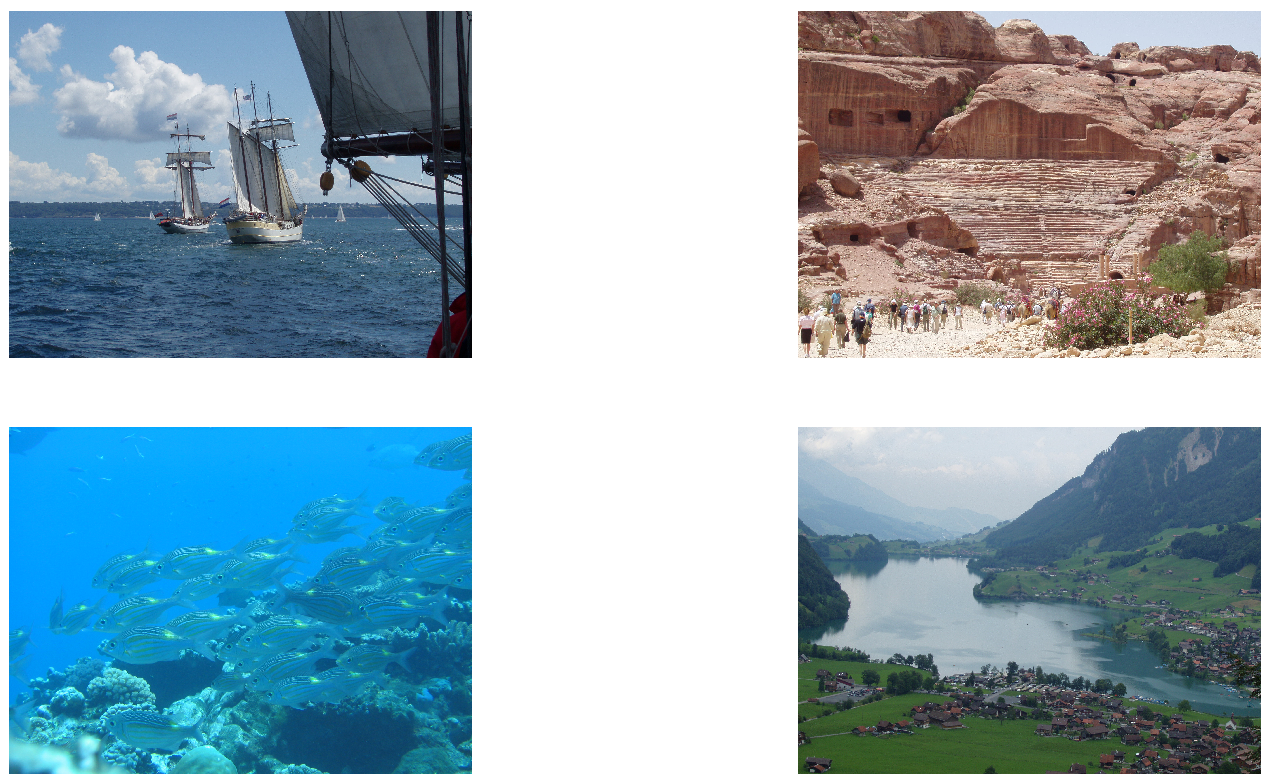
\includegraphics[width=6in]{dataset_filters}
      \caption[Przykładowe obrazy ze zbioru treningowego - źródło: Praca własna]{Przykładowe obrazy ze zbioru treningowego}
      \label{fig:dataset_filters}
    \end{figure}

    Aby mogły właściwie pełnić swoją rolę obrazy treningowe zostały w pierwszej kolejności
    poddane odpowiedniemu przetworzeniu wstępnemu. W ramach tego procesu rozmiar każdego zdjęcia
    zmniejszony został do wymiarów $256x256$ pikseli, a wartości kolorów ograniczone
    do zakresu $<0, 1>$ w celu usprawnienia obliczeń wykonywanych przez sieć m.in.
    poprzez zapobieganie zjawisku eksplodującego gradientu. Dodatkowo w przypadku tego
    filtru zastosowana została konwersja obrazów do formatu czarno-białego, co pozwoliło
    wyodrębnić pojedynczy kanał kolorystyczny z oryginałów. Tak przetworzony zbiór uczący
    podawany był na wejście sieci neuronowej, a rezultaty jej pracy porównywane
    z obrazami na które dodatkowo nałożony został filtr Sobela za pomocą biblioteki
    \textit{OpenCV}. W przypadku obrazów referencyjnych po zastosowaniu filtracji
    konieczne okazało się również przeskalowanie wartości pikseli do przedziału
    $<0, 1>$, ponieważ w sieci zastosowana została funkcja aktywacji \textit{ReLU}, która
    opisana została w rozdziale \ref{funkcje_aktywacji}. Jej charakterystyka
    wyklucza pojawianie się wartości ujemnych, jako rezultatów pracy modelu, co
    w przypadku braku odpowiedniej normalizacji prowadziło do niepoprawnych wyników.

    Sam model sieci składa się w tym przypadku z pojedynczegwo neuronu w warstwie
    konwolucyjnej, filtrującego obraz za pomocą macierzy kwadratowej stopnia
    trzeciego. Odzwierciedla to oryginalną macierz filtracji $G_x$ w stosunku jeden
    do jednego, ponieważ każda z dziewięciu wag sieci odpowiada jednemu polu w tej
    macierzy. Takie podejście pozwala jednoznacznie ocenić stopień odwzorowania
    maski przez sieć poprzez analizę wartości jej parametrów.

    W ramach przeprowadzonych eksperymentów, wypróbowane zostały różne konfiguracje
    hiperparametrów treningowych. Ostatecznie najlepszy rezultat udało się uzyskać
    przy zastosowaniu następującej konfiguracji:

    \begin{itemize}
    \item Funkcja kosztu: \textit{SmoothL1Loss}
    \item Optymalizator: \textit{Adam}
    \item Funkcja aktywacji: \textit{ReLU}
    \item Ilość epok treningowych: 3
    \item Rozmiar pakietu danych: 8
    \end{itemize}

    Efekt działania wytrenowanego modelu przedstawia Rysunek \ref{fig:sobel_result}.

    \begin{figure}[H]
      \centering
      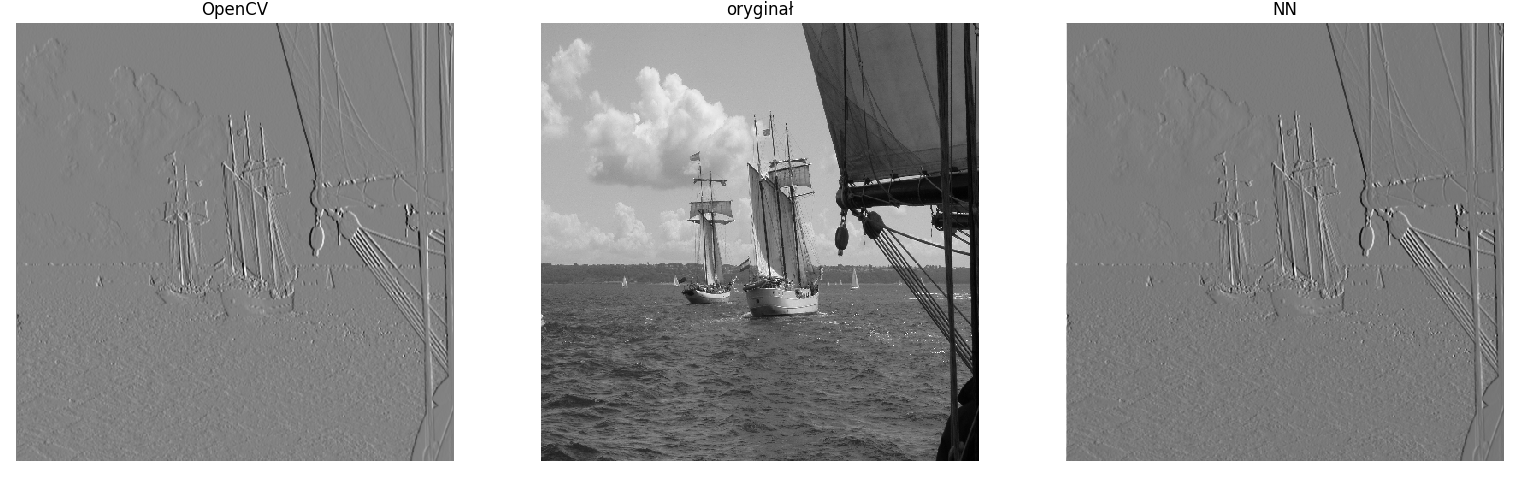
\includegraphics[width=6in]{sobel_result}
      \caption[Działanie filtru Sobela - źródło: Praca własna]{Działanie filtru Sobela}
      \label{fig:sobel_result}
    \end{figure}

    Zgodnie z opisem oryginalne, czarno-białe zdjęcie poddawane filtracji zamieszczone
    zostało na środku. Po lewej stronie przedstawiony został obraz przefiltrowany
    z wykorzystaniem biblioteki \textit{OpenCV}, a po prawej obraz przetworzony przez
    wytrenowany model sieci neuronowej. Wizualnie otrzymane rezultaty są niemal
    identyczne. Zdjęcie wygenerowane przez sieć charakteryzuje się nieco ciemniejszą
    barwą, co może mieć związek z normalizacją danych przeprowadzaną w celu skuteczniejszego
    uczenia sieci. Poprawne rezultaty treningu najlepiej ocenić można analizując
    macierz wag modelu, która przedstawia się następująco:

    \[G_{nn} =
    \begin{bmatrix}
    -0.1135 & -0.0144 & +0.1363 \\
    -0.3239 & -0.0016 & +0.3340 \\
    -0.1199 & -0.0058 & +0.1335
    \end{bmatrix}
    \]

    Porównując uzyskane rezultaty z oryginalną maską $G_x$ łatwo zauważyć można,
    że sieć neuronowa właściwie odtworzyła panujące w niej proporcje. Odpowiednio
    mniejszy rząd wielkości odzwierciedla normalizację danych na których uczony
    był model. Środkowa kolumna składa się w całości z wartości bliskich zeru.
    Kolumna prawa zawiera wartości dodatnie z wyraźną dominacją elementu środkowego.
    Podobnie rozkładają się wartości w kolumnie lewej zawierającej wyłącznie wartości
    ujemne.

    Wskazówką w określaniu poprawności przeprowadzanych treningów może być również
    wykres wartości funkcji kosztu w kolejnych krokach uczenia. Przebieg taki
    przedstawiony został na Rysunku \ref{fig:tensorboard_sobel}.

    \begin{figure}[H]
      \centering
      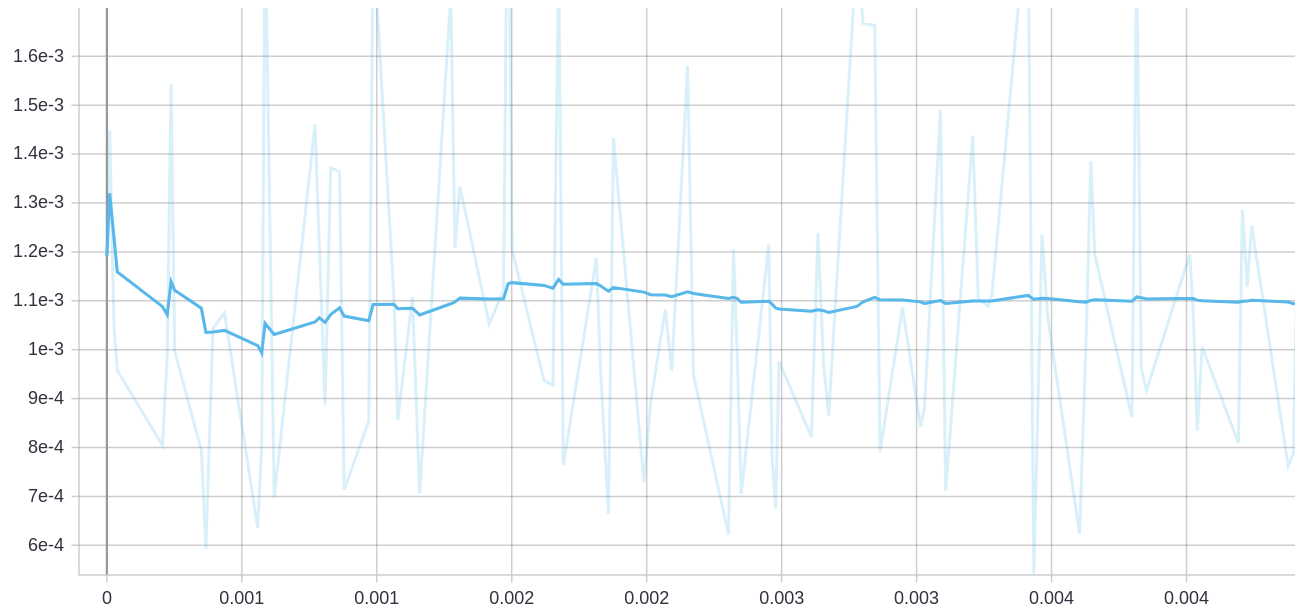
\includegraphics[width=6in]{tensorboard_sobel}
      \caption[Wykres wartości funkcji kosztu w zależności od ilości kroków treningowych - źródło: Praca własna]{Wykres wartości funkcji kosztu w zależności od ilości kroków treningowych}
      \label{fig:tensorboard_sobel}
    \end{figure}

    W początkowej fazie przedstawiona charakterystyka cechuje się znaczącym spadkiem
    wartości, po czym utrzymuje się na stosunkowo stałym poziomie. Jest to spodziewany
    efekt, spowodowany niewielkimi rozmiarami modelu, co przełożyło się na szybkie
    zlokalizowanie globalnego minimum przez zastosowany optymalizator. Warto wspomnieć,
    że zastosowanie tej metryki do analizy działania sieci może być zwodnicze.
    Ciągły spadek wartości funkcji kosztu nie zawsze oznacza wzrost dokładności działania
    trenowanego modelu. Sieć neuronowa może zacząć w zbyt dużym stopniu dostosowywać się
    do dostępnych danych treningowych tracąc zdolność do generalizacji rozwiązania dla
    przykładów spoza tego zbioru. Zjawisko takie nazywane jest przeuczeniem i najczęściej
    objawia się spadkiem dokładności, przy jednoczesnym opadaniu wartości funkcji kosztu.

    Liczne eksperymenty związane z zastosowaniem rozmaitych hiperparametrów wykazały, że
    pomimo niewielkich rozmiarów modelu zlokalizowanie minimum globalnego nie było
    zadaniem trywialnym. Prosty optymalizator, taki jak \textit{SGD} nie był w stanie odnaleźć
    odpowiedniego punktu, a rezultaty jego działania w dużej mierze zależały od
    losowych wartości przypisanych do wag sieci na początku każdej sesji treningowej.
    Dopiero zastosowanie algorytmu adaptacyjnego, jakim jest \textit{Adam} pozwoliło
    uzyskać powtarzalność w osiąganiu właściwych rezultatów. Algorytm \textit{SGD}
    zastosowany został dopiero w końcowej fazie uczenia z bardzo małym krokiem
    treningowym rzędu $\eta = 10^{-8}$, co pozwoliło nieznacznie poprawić uzyskane
    wyniki.

    Olbrzymi wpływ na rezultaty miały również zastosowane sposoby przetworzenia danych
    treningowych, między innymi wspomniane już ograniczenie wartości pikseli
    w przedziale $<0,1>$, tak aby współgrały z zastosowaną funckją aktywacji.

  \subsubsection{Sepia}

    Sepia to filtr obrazu nadający zdjęciom charakterystycznego czerwonawo-brązowego
    koloru. Jego nazwa pochodzi od rodzaju mątwy, Sepii, z której pozyskiwany
    był atrament cechujący się takim właśnie zabarwieniem. Choć obecnie materiał ten
    nie jest już powszechnie wykorzystywany w malarstwie, to sepia wciąż cieszy się
    sporą popularnością w dziedzinie fotografii i cyfrowego przetwarzania obrazów.

    Zastosowanie sepii, jako filtru, wiąże się z konwolucyjnym przetworzeniem
    zdjęcia za pomocą następującej maski:

    \[G_x =
    \begin{bmatrix}
    +0.131 & +0.534 & +0.272 \\
    +0.168 & +0.686 & +0.349 \\
    +0.189 & +0.769 & +0.393
    \end{bmatrix}
    \]

    Sieć neuronowa użyta do jej odtworzenia składa się z trzech neuronów w
    warstwie splotowej. Jest to minimalna struktura niezbędna do odtworzenia
    trójkanałowego obrazu wyjściowego, jako że każdy filtr odpowiada za wygenerowanie
    pojedynczej warstwy kolorystycznej.

    W procesie uczenia sieci zastosowany został identyczny zbiór treningowy, co w
    przypadku filtru Sobela, opisanego w poprzednim rozdziale. Ponownie w ramach
    wstępnego przetwarzania danych, wartości pikseli ograniczone zostały w przedziale
    $<0,1>$, a każdy obraz przeskalowany do wymiarów $256x256$. W przypadku obrazów
    referencyjnych zastosowany został oczywiście filtr zapewniający efekt sepii
    pochodzący z biblioteki \textit{OpenCV}. Dodatkowo wartości, które w wyniku filtracji
    przekroczyły wartość 1, zostały ograniczone do jej poziomu. Główną różnicą w stosunku
    do opisanego uprzednio filtru Sobela jest fakt, że sieć trenowana była na
    obrazach posiadających pełny zakres trzech kanałów kolorystycznych, a nie jak
    poprzednio z wykorzystaniem formatu czarno-białego.

    Optymalny rezultat działania sieci udało się uzyskać dla następującego
    zestawu hiperparametrów:

    \begin{itemize}
    \item Funkcja kosztu: \textit{SmoothL1Loss}
    \item Optymalizator: \textit{Adam}
    \item Funkcja aktywacji: \textit{ReLU}
    \item Ilość epok treningowych: 5
    \item Rozmiar pakietu danych: 8
    \end{itemize}

    Większość parametrów nie uległa zmianie w stosunku do filtru Sobela. Świadczy to
    przede wszystkim o uniwersalności algorytmu \textit{Adam} w odnajdywaniu optymalnych
    rozwiązań w procesie minimalizacji. Rezultaty pracy wytrenowanego modelu przedstawione
    zostały na Rysunku \ref{fig:sepia_result}.

    \begin{figure}[H]
      \centering
      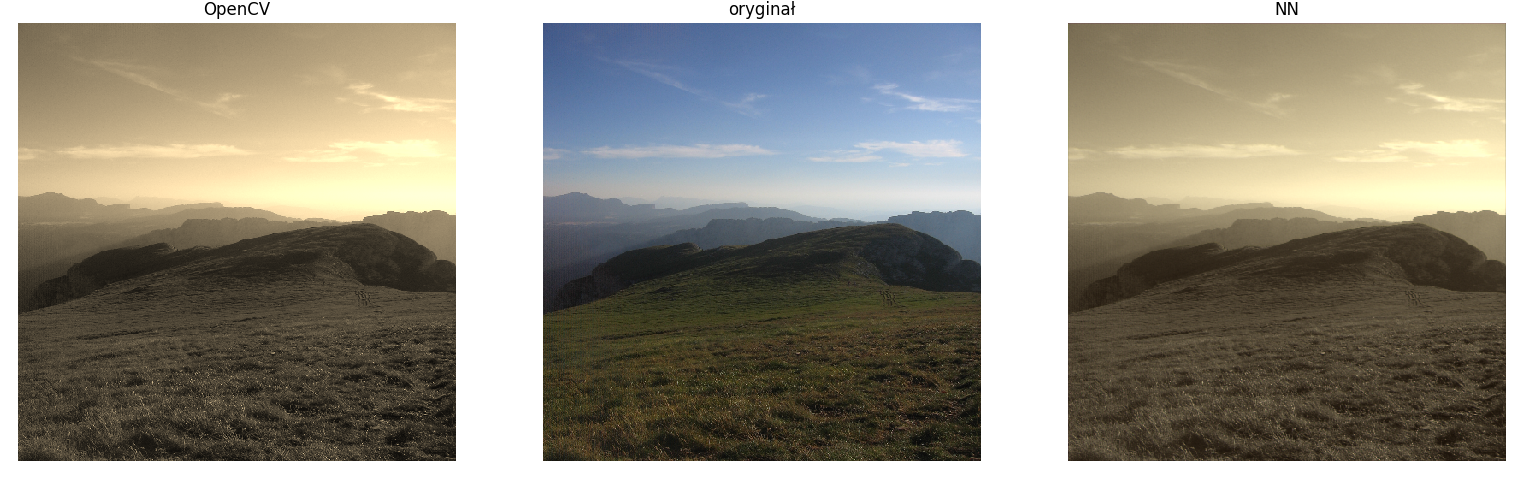
\includegraphics[width=6in]{sepia_result}
      \caption[Działanie sepii - źródło: Praca własna]{Działanie sepii}
      \label{fig:sepia_result}
    \end{figure}

    Wizualnie wyniki działania sztucznej sieci neuronowej cechują się nieco bardziej
    przytłumionymi kolorami w stosunku do obrazów wygenerowanych z wykorzystaniem
    oryginalnej maski. Powodem takiego zachowania jest najprawdopodobniej dążenie
    sieci do zminimalizowania wartości funkcji kosztu w obrębie całego zbioru
    treningowego, co wiąże się z pewnym mimowolnym uśrednieniem wag modelu. Przekłada
    się ono na trudności w odwzorowaniu obrazów cechujących się dużym kontrastem.

    Dodatkowo w rozważanym przypadku rozmiar zastosowanej sieci, choć pozornie
    niewielki, nie pozwala jednoznacznie przełożyć uzyskanych parametrów modelu na
    referencyjną maskę $G_x$. Każdy z trzech zastosowanych filtrów przetwarza
    obraz za pomocą macierzy $3x3$ dla każdej z trzech warstw kolorystycznych.
    Oznacza to, że pojedynczy neuron powiązany jest z 27 wagami, a w całym modelu
    jest ich sumarycznie 81. Informacja o sposobie filtracji jest więc mocno
    rozproszona i ciężko jednoznacznie odczytać postać maski jaką w praktyce
    implementuje wytrenowany model.

    W takiej sytuacji, poza wizualną oceną działania sieci, przydatnych informacji
    dostarcza wykres wartości funkcji kosztu przedstawiony na Rysunku \ref{fig:tensorboard_sepia}.

    \begin{figure}[H]
      \centering
      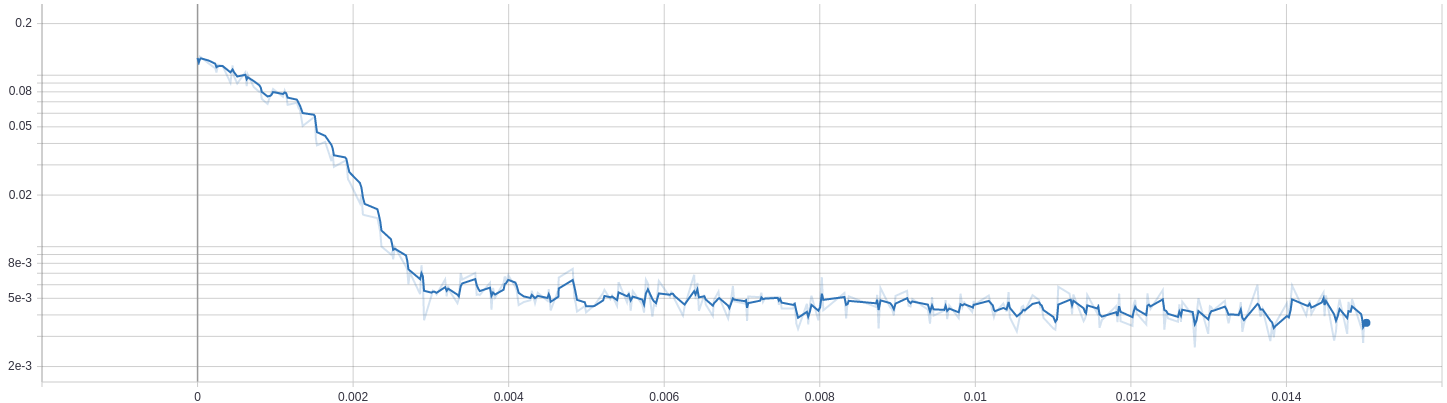
\includegraphics[width=6in]{tensorboard_sepia}
      \caption[Wykres wartości funkcji kosztu w zależności od ilości kroków treningowych - źródło: Praca własna]{Wykres wartości funkcji kosztu w zależności od ilości kroków treningowych}
      \label{fig:tensorboard_sepia}
    \end{figure}

    Wyraźne zbocze opadające w początkowej fazie treningu świadczy o poprawnym dążeniu
    sieci do rozwiązania optymalnego, a następujące po nim wypłaszczenie oznacza, że
    rozwiązanie to zostało osiągnięte. Porównując Rysunki \ref{fig:tensorboard_sepia}
    i \ref{fig:tensorboard_sobel} zauważyć można że w przypadku sepii długość zbocza
    opadającego jest znacząco większa. Może być to spowodowane większą złożonością
    funkcji kosztu w przypadku tego filtru, lub niekorzystnym początkowym umiejscowieniem
    algorytmu optymalizacji na płaszczyźnie celu, wynikającym z losowego doboru startowych parametrów sieci.
    Najprawdopodobniej oba te czynniki wywarły swój wpływ na przebieg procesu uczenia.

    W ramach przeprowadzonych eksperymentów ponownie testowane były rozmaite funkcje
    optymalizacji, jednak żadna nie pozwoliła osiągnąć takiej powtarzalności w osiąganiu
    poprawnych rezultatów, jak \textit{Adam}. Nawet zastosowanie innych optymalizatorów
    adaptacyjnych bardzo często kończyło się na osiągnięciu jedynie jednego z minimów
    lokalnych. Przykładem takiego rozwiązania może być efekt działania algorytmu
    \textit{Adagrad} przedstawiony na Rysunku \ref{fig:sepia_fail}.

    \begin{figure}[H]
      \centering
      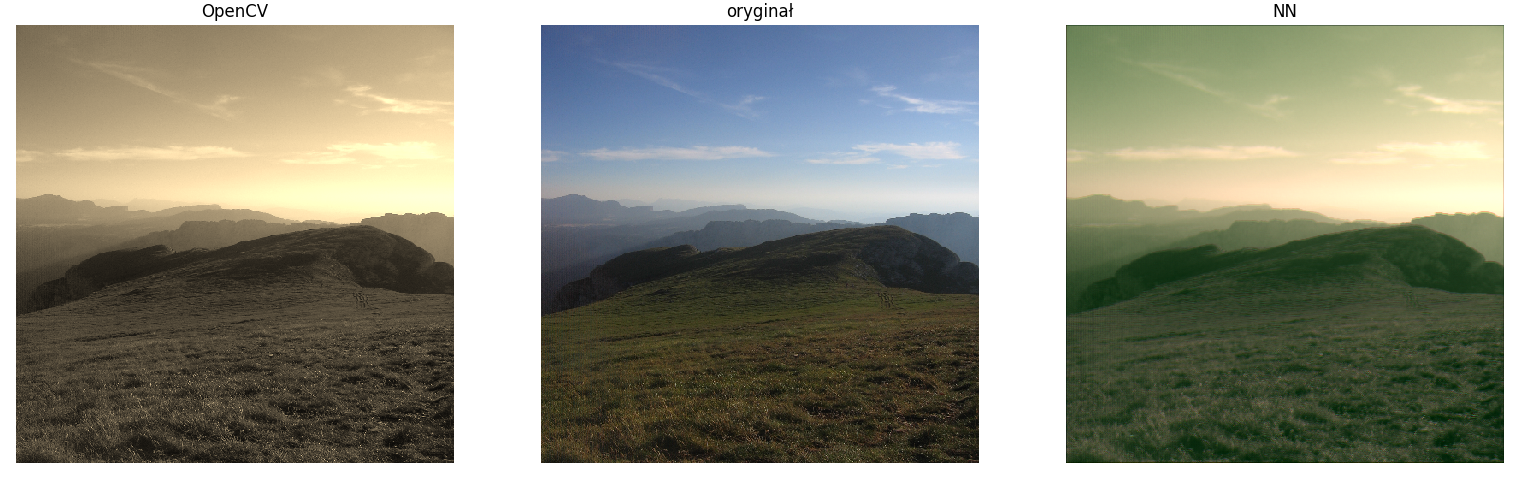
\includegraphics[width=6in]{sepia_fail}
      \caption[Przykład działania sieci w minimum lokalnym - źródło: Praca własna]{Przykład działania sieci w minimum lokalnym}
      \label{fig:sepia_fail}
    \end{figure}

    Choć na obrazie wygenerowanym przez sieć dostrzec można pewne podobieństwo do
    poprawnie działającego filtru, to wyraźnie widać że nie jest to zadowalający
    rezultat, a znalezione na hiperpłaszczyźnie funkcji celu minimum nie jest z pewnością
    minimum globalnym.

  \subsubsection{Filtr górnoprzepustowy}

    Filtry górnoprzepustowe używane są w celu uwypuklenia szczegółów występujących na
    obrazie. Tłumią one elementy o niskiej częstotliwości, a wzmacniają te cechujące
    się częstotliwościami wysokimi poprzez zwiększenie ich jasności lub barwy.
    Efektem zastosowania filtru górnoprzepustowego jest najczęściej zwiększenie
    kontrastu poprzez podkreślenie ostrych krawędzi obiektów. W pracy
    \textit{"Image Enhancement Techniques using Highpass and
    Lowpass Filters"} \cite{highpass_filter} znaleźć można następujący opis:

    \begin{quote}
      "Filtr górnoprzepustowy to filtr, który dobrze przepuszcza wysokie częstotliwości,
      ale tłumi częstotliwości niższe niż częstotliwość graniczna. Ostrzenie jest
      zasadniczo operacją górnoprzepustową w dziedzinie częstotliwości.

      Istnieje kilka standardowych form filtrów górnoprzepustowych, takich jak
      filtr Butterworth'a, czy Gauss'a. Wszystkie filtry górnoprzepustowe ($H_{hp}$) są
      zazwyczaj reprezentowane poprzez ich relację z filtrami dolnoprzepustowymi ($H_{lp}$):

      \[H_{hp} = 1 - H_{lp}\]."
    \end{quote}

    W ramach niniejszego eksperymentu zastosowany został filtr górnoprzepustowy
    reprezentowany przez maskę następującej postaci:

    \[G_x =
    \begin{bmatrix}
    -1 & -1 & -1 \\
    -1 & +9 & -1 \\
    -1 & -1 & -1
    \end{bmatrix}
    \]

    W celu odwzorowania działania filtru zastosowana została sztuczna sieć
    splotowa złożona z trzech neuronów, podobnie jak miało to miejsce w przypadku
    sepii. Model sieci uczony był na tych samych danych, z tą różnicą, że dane
    referencyjne zostały przetworzone z wykorzystaniem filtru górnoprzepustowego
    $G_x$.

    Wyniki działania wytrenowanego modelu przedstawia Rysunek \ref{fig:sharpen_result}.

    \begin{figure}[H]
      \centering
      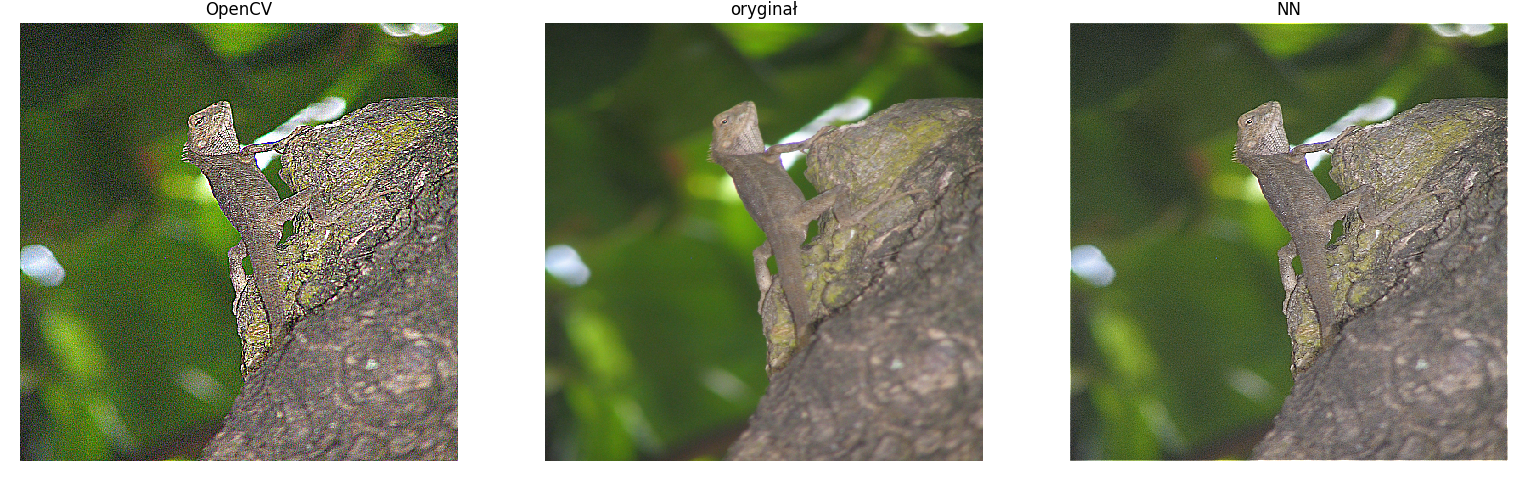
\includegraphics[width=6in]{sharpen_result}
      \caption[Działanie filtru górnoprzepustowego - źródło: Praca własna]{Działanie filtru górnoprzepustowego}
      \label{fig:sharpen_result}
    \end{figure}

    Parametry dla których uzyskany został przedstawiony efekt są następujące:

    \begin{itemize}
    \item Funkcja kosztu: \textit{SmoothL1Loss}
    \item Optymalizator: \textit{Adam}
    \item Funkcja aktywacji: \textit{ReLU}
    \item Ilość epok treningowych: 5
    \item Rozmiar pakietu danych: 2
    \end{itemize}

    Na uwagę zasługuje tutaj przede wszystkim rozmiar pakietu danych odróżniający
    ten zbiór hiperparametrów od dwóch poprzednich. Został on zmniejszony w celu
    ograniczenia wpływu uśrednienia wartości funkcji kosztu na modyfikację wag
    modelu. Pomimo tego zabiegu wyraźnie widać, że w ramach wszystkich przeprowadzonych
    eksperymentów to właśnie efekt działania sieci górnoprzepustowej najbardziej
    odbiega od obrazu referencyjnego. Jest to spowodowane charakterem działania
    badanego filtru. Jego celem jest uwypuklanie pojedynczych elementów obrazu, takich
    jak krawędzie, co stoi w niejakiej sprzeczności z procesem treningu, którego celem
    jest osiągnięcie jak najmniejszej wartości błędu w obrębie wszystkich danych
    treningowych. Oznacza to, że sieć będzie dążyła do jak najlepszego uśrednienia
    procesu filtracji górnoprzepustowej. Efekt ten został niewątpliwie osiągnięty.
    Obraz wygenerowany przez model cechuje się wyraźniejszymi konturami, jednak
    nie w takim stopniu jak obraz docelowy.

    Wykres wartości funkcji kosztu przedstawia Rysunek \ref{fig:tensorboard_sharpen}.

    \begin{figure}[H]
      \centering
      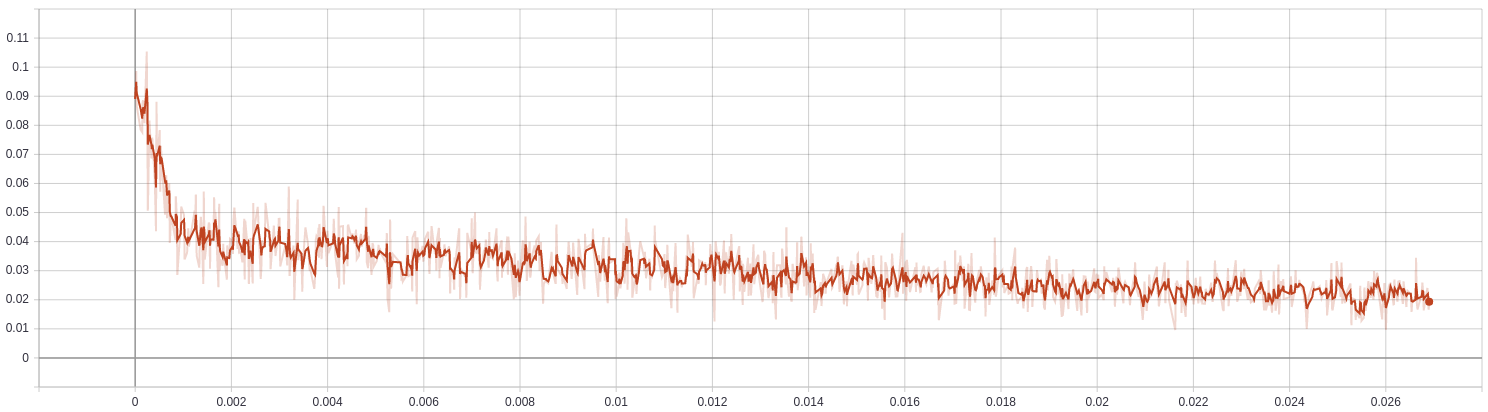
\includegraphics[width=6in]{tensorboard_sharpen}
      \caption[Wykres wartości funkcji kosztu w zależności od ilości kroków treningowych - źródło: Praca własna]{Wykres wartości funkcji kosztu w zależności od ilości kroków treningowych}
      \label{fig:tensorboard_sharpen}
    \end{figure}

    Podobnie jak w dwóch poprzednich przypadkach początkowy spadek wartości
    prowadzi model do punktu optymalnego rozwiązania. W punkcie tym algorytm optymalizacji
    zaczyna nieznacznie oscylować podejmując kolejne próby poprawy uzyskanych wyników.

    W ramach testów różnych rozwiązań na uwagę zasługują rezultaty osiągnięte
    z wykorzystaniem optymalizatora \textit{AdaDelta} przedstawione na Rysunku \ref{fig:sharpen_fail}.

    \begin{figure}[H]
      \centering
      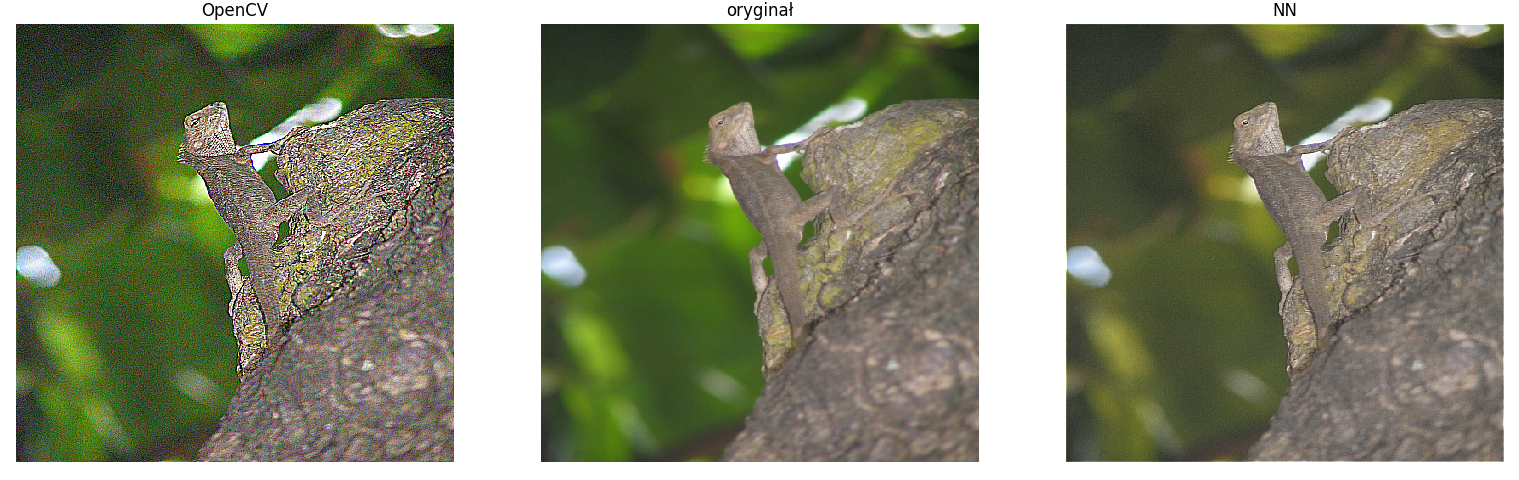
\includegraphics[width=6in]{sharpen_fail}
      \caption[Przykład działania sieci w minimum lokalnym - źródło: Praca własna]{Przykład działania sieci w minimum lokalnym}
      \label{fig:sharpen_fail}
    \end{figure}

    Wygenerowany obraz został wyostrzony w stosunku do oryginału, jednak
    nieznacznie wypaczone zostały przy tym kolory tła, co jest zjawiskiem niekorzystnym i
    może wskazywać na osiągnięcie przez model jednego z lokalnych minimów funkcji celu.

  \subsubsection{Podsumowanie}

    Przeprowadzone w ramach tego rozdziału eksperymenty dowodzą, że sztuczne
    sieci splotowe z powodzeniem mogą posłużyć w procesie filtrowania obrazów.
    Należy zadać sobie jednak pytanie, czy rezultaty ich działania są w stanie
    zrekompensować stosunkowo czasochłonny proces treningu związany z odpowiednią
    obróbką danych oraz eksperymentalnym doborem właściwych hiperparametrów.

    W przypadku prostych filtrów, jak sepia, czy filtr górnoprzepustowy korzystniejsze
    okazuje się zastosowanie klasycznych metod przetwarzania w postaci
    odpowiednich masek konwolucyjnie nakładanych na docelowe obrazy. Rozwiązania te
    są często pozbawione typowej dla sieci neuronowych tendencji do uśredniania
    wyników, co przekłada się na lepsze rezultaty w sytuacjach, w których celem jest
    na przykład osiągnięcie dużego kontrastu przetwarzanych obrazów.

    Nie oznacza to jednak, że sieci neuronowe mogą zostać zastąpione w każdej sytuacji.
    Ich zdolności adaptacyjne sprawiają, że znajdują one zastosowanie w rozwiązaniach, w
    których klasyczne metody zawodzą. Dowodem na to będą kolejne rozdziały tej pracy.
